\documentclass[tikz,border=12pt]{standalone}
\usepackage[T1]{fontenc}
\usepackage{tgheros}
\usepackage{sfmath}
\usepackage{amsmath}
\usepackage{amssymb}
% % \usepackage{fontawesome5} (Removed for publication-grade academic typography) (Removed for publication-grade academic typography)
\usepackage{tikz}
\usetikzlibrary{arrows.meta,positioning,shapes.geometric,fit,backgrounds,calc}
\usepackage{xcolor}

\renewcommand{\familydefault}{\sfdefault}

% Academic Semantic Palette
\definecolor{harvardcrimson}{HTML}{A51C30}
\definecolor{ethdarkblue}{HTML}{1F407A}
\definecolor{ethblue}{HTML}{215CAF}
\definecolor{ethpetrol}{HTML}{007A87}
\definecolor{ethbronze}{HTML}{B87333}
\definecolor{ethpurple}{HTML}{5B4B8A}
\definecolor{ethslate}{HTML}{475569}
\definecolor{cardbg}{HTML}{F8FAFC}
\definecolor{cardborder}{HTML}{CBD5E1}
\definecolor{safeTeal}{HTML}{10B981}
\definecolor{proposalAmber}{HTML}{C98218}

\begin{document}
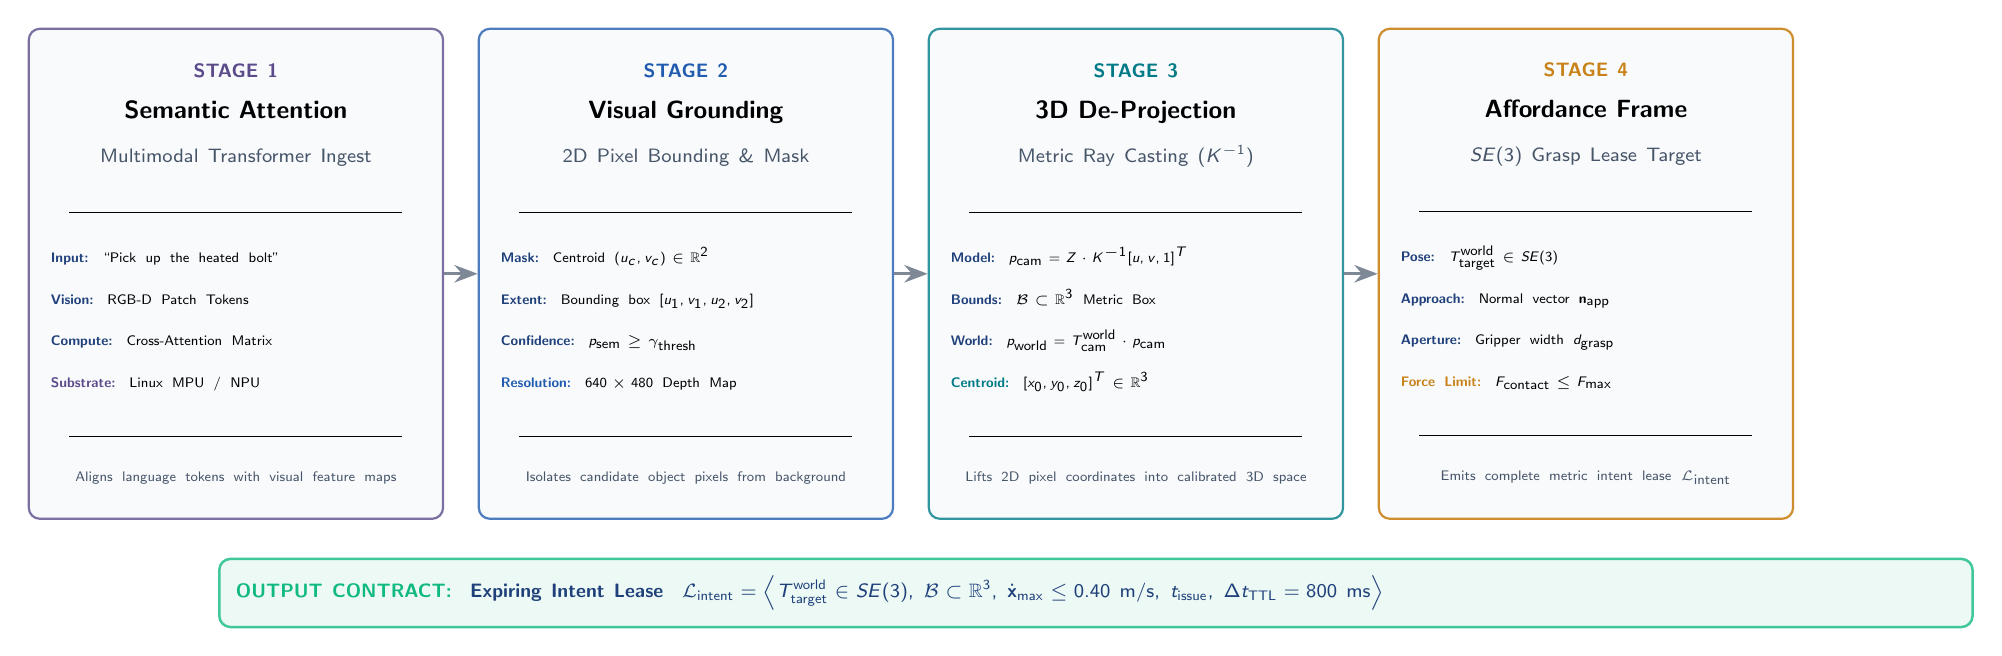
\begin{tikzpicture}[
  font=\sffamily,
  >=Stealth,
  stagecard/.style={
    draw=cardborder,
    fill=cardbg,
    rounded corners=4pt,
    line width=0.8pt,
    text width=1.85in,
    minimum height=2.45in,
    inner sep=8pt,
    align=center,
    anchor=north
  }
]

  % Top Title Banner
  % (Top title banner removed for academic publication standards)
% Stage 1: Linguistic Prompt & Visual Attention
  \node[stagecard, draw=ethpurple!80] (st1) at (0, 0.00in) {
    {\scriptsize\bfseries\color{ethpurple} STAGE 1}\\[3pt]
    {\small\bfseries Semantic Attention}\\[4pt]
    {\scriptsize\color{ethslate}Multimodal Transformer Ingest}\\[6pt]
    \rule{0.9\linewidth}{0.3pt}\\[6pt]
    \raggedright
    {\tiny\textbf{\color{ethdarkblue}Input:} \mbox{``Pick up the heated bolt''}}\\[3pt]
    {\tiny\textbf{\color{ethdarkblue}Vision:} RGB-D Patch Tokens}\\[3pt]
    {\tiny\textbf{\color{ethdarkblue}Compute:} Cross-Attention Matrix}\\[3pt]
    {\tiny\textbf{\color{ethpurple}Substrate:} Linux MPU / NPU}\\[6pt]
    \centering
    \rule{0.9\linewidth}{0.3pt}\\[4pt]
    {\tiny\color{ethslate}Aligns language tokens with visual feature maps}
  };

  % Stage 2: 2D Segmentation & Patch Masking
  \node[stagecard, draw=ethblue!80] (st2) at (2.25in, 0.00in) {
    {\scriptsize\bfseries\color{ethblue} STAGE 2}\\[3pt]
    {\small\bfseries Visual Grounding}\\[4pt]
    {\scriptsize\color{ethslate}2D Pixel Bounding \& Mask}\\[6pt]
    \rule{0.9\linewidth}{0.3pt}\\[6pt]
    \raggedright
    {\tiny\textbf{\color{ethdarkblue}Mask:} Centroid $(u_c, v_c) \in \mathbb{R}^2$}\\[3pt]
    {\tiny\textbf{\color{ethdarkblue}Extent:} Bounding box $[u_1, v_1, u_2, v_2]$}\\[3pt]
    {\tiny\textbf{\color{ethdarkblue}Confidence:} $p_{\text{sem}} \ge \gamma_{\text{thresh}}$}\\[3pt]
    {\tiny\textbf{\color{ethblue}Resolution:} $640 \times 480$ Depth Map}\\[6pt]
    \centering
    \rule{0.9\linewidth}{0.3pt}\\[4pt]
    {\tiny\color{ethslate}Isolates candidate object pixels from background}
  };

  % Stage 3: Depth De-projection (K^-1)
  \node[stagecard, draw=ethpetrol!80] (st3) at (4.50in, 0.00in) {
    {\scriptsize\bfseries\color{ethpetrol} STAGE 3}\\[3pt]
    {\small\bfseries 3D De-Projection}\\[4pt]
    {\scriptsize\color{ethslate}Metric Ray Casting ($K^{-1}$)}\\[6pt]
    \rule{0.9\linewidth}{0.3pt}\\[6pt]
    \raggedright
    {\tiny\textbf{\color{ethdarkblue}Model:} $p_{\text{cam}} = Z \cdot K^{-1} [u, v, 1]^T$}\\[3pt]
    {\tiny\textbf{\color{ethdarkblue}Bounds:} $\mathcal{B} \subset \mathbb{R}^3$ Metric Box}\\[3pt]
    {\tiny\textbf{\color{ethdarkblue}World:} $p_{\text{world}} = T_{\text{cam}}^{\text{world}} \cdot p_{\text{cam}}$}\\[3pt]
    {\tiny\textbf{\color{ethpetrol}Centroid:} $[x_0, y_0, z_0]^T \in \mathbb{R}^3$}\\[6pt]
    \centering
    \rule{0.9\linewidth}{0.3pt}\\[4pt]
    {\tiny\color{ethslate}Lifts 2D pixel coordinates into calibrated 3D space}
  };

  % Stage 4: SE(3) Affordance Framing
  \node[stagecard, draw=proposalAmber!90] (st4) at (6.75in, 0.00in) {
    {\scriptsize\bfseries\color{proposalAmber} STAGE 4}\\[3pt]
    {\small\bfseries Affordance Frame}\\[4pt]
    {\scriptsize\color{ethslate}$SE(3)$ Grasp Lease Target}\\[6pt]
    \rule{0.9\linewidth}{0.3pt}\\[6pt]
    \raggedright
    {\tiny\textbf{\color{ethdarkblue}Pose:} $T_{\text{target}}^{\text{world}} \in SE(3)$}\\[3pt]
    {\tiny\textbf{\color{ethdarkblue}Approach:} Normal vector $\mathbf{n}_{\text{app}}$}\\[3pt]
    {\tiny\textbf{\color{ethdarkblue}Aperture:} Gripper width $d_{\text{grasp}}$}\\[3pt]
    {\tiny\textbf{\color{proposalAmber}Force Limit:} $F_{\text{contact}} \le F_{\text{max}}$}\\[6pt]
    \centering
    \rule{0.9\linewidth}{0.3pt}\\[4pt]
    {\tiny\color{ethslate}Emits complete metric intent lease $\mathcal{L}_{\text{intent}}$}
  };

  % Connecting Arrows Between Stages
  \draw[->, line width=1.2pt, draw=ethslate!70] (st1.east) -- (st2.west);
  \draw[->, line width=1.2pt, draw=ethslate!70] (st2.east) -- (st3.west);
  \draw[->, line width=1.2pt, draw=ethslate!70] (st3.east) -- (st4.west);

  % Bottom Output Summary Strip
  \node[draw=safeTeal!80, fill=safeTeal!8, rounded corners=4pt, line width=0.9pt, text width=8.60in, inner sep=6pt, anchor=north] (summary) at (4.30in, -2.65in) {
    \centering
    {\scriptsize\bfseries\color{safeTeal} OUTPUT CONTRACT:}
    {\scriptsize\color{ethdarkblue}\textbf{ Expiring Intent Lease } $\mathcal{L}_{\text{intent}} = \left\langle T_{\text{target}}^{\text{world}} \in SE(3), \; \mathcal{B} \subset \mathbb{R}^3, \; \dot{\mathbf{x}}_{\text{max}} \le 0.40\text{ m/s}, \; t_{\text{issue}}, \; \Delta t_{\text{TTL}} = 800\text{ ms} \right\rangle$}
  };

\end{tikzpicture}
\end{document}
